%% LyX 2.0.0 created this file.  For more info, see http://www.lyx.org/.
%% Do not edit unless you really know what you are doing.
\documentclass[ngerman]{article}
\usepackage[latin9]{inputenc}
\usepackage{listings}
\usepackage{geometry}
\geometry{verbose,tmargin=2cm,bmargin=2cm,lmargin=1.5cm,rmargin=1.5cm}
\usepackage{babel}
\usepackage{url}
\usepackage{graphicx}
\usepackage[unicode=true,pdfusetitle,
 bookmarks=true,bookmarksnumbered=false,bookmarksopen=false,
 breaklinks=false,pdfborder={0 0 1},backref=false,colorlinks=false]
 {hyperref}
\usepackage{breakurl}
\begin{document}
\selectlanguage{ngerman}

\section{Elexis OpenVPN-Client f�r Analytica}

Mit diesem Plug-In lassen sich einfach Labordaten von Analytica �bernehmen.
Wir zeigen hier auf, wie Sie OpenVPN installieren, das Plugin-Konfigurieren
und einen Import durchf�hren.


\subsection{Installation des Windows-OpenVPN-Clients}

Falls Ihr Support OpenVPN schon auf Ihrem Computer installiert hat,
sollten Sie in Ihrer Bildschirmleiste das Icon von {}``OpenVPN''
sehen (in dieser Abbildung in der Mitte).

~


\includegraphics{images/OpenVPN_Config_1}\\


Falls dies der Fall ist, �berspringen Sie diesen Abschnitt.

OpenVPN kann vom Internet aus \href{ http://www.openvpn.net/release/openvpn-2.1.1-install.exe}{http://www.openvpn.net/index.php/open-source/downloads.html}
hinuntergeladen werden. Bei diesen Beispielen wurde eine englische
Version gebraucht. 
\begin{description}
\item [{{�bersetzte}}] Versionen findet man f�r

\begin{description}
\item [{{Deutsch}}] http://openvpn.se/files/localized/binary/1.0.3/openvpn-gui-1.0.3-de.exe 
\item [{{Franz�sich}}] http://openvpn.se/files/localized/binary/1.0.3/openvpn-gui-1.0.3-fr.exe 
\item [{{Italienisch}}] http://openvpn.se/files/localized/binary/1.0.3/openvpn-gui-1.0.3-it.exe 
\end{description}
\end{description}
Wir nehmen im folgenden an, dass Sie diese unter C:\textbackslash{}Programme\textbackslash{}OpenVPN
installiert haben

Diese Datei ausf�hren (allf�llige Warnungen quittieren). Dann sollte
folgendes Fenster erscheinen:

~

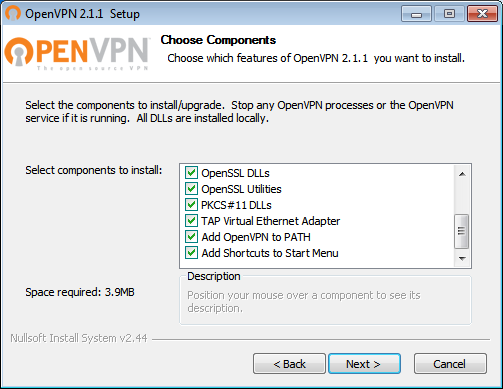
\includegraphics[scale=0.5]{images/OpenVPN_Setup_1}\\


Auf Next dr�cken.\newpage{}Beim n�chsten Dialog muss der Pfad angegeben
werden. Falls Sie sich f�r einen anderen entscheiden, m�ssen Sie Sich
diesen merken, da er sp�ter bei der Konfiguration des Plugins gebraucht
wird.~\\
 ~

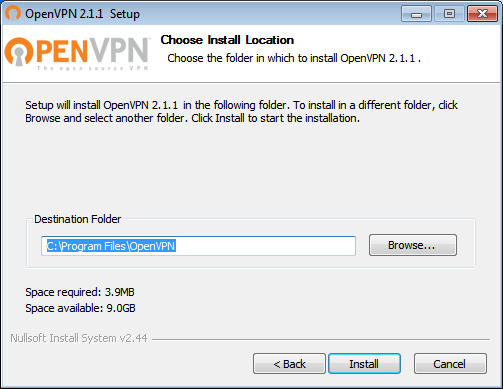
\includegraphics[scale=0.5]{images/OpenVPN_Setup_2}\\


Nach dem Dr�cken auf Install geht es eine Weile, bis alle Datein kopiert
wurden. Warten, bis {}``Installation Complete'' erscheint und die
Taste {}``Next'' gedr�ckt werden kann.

~

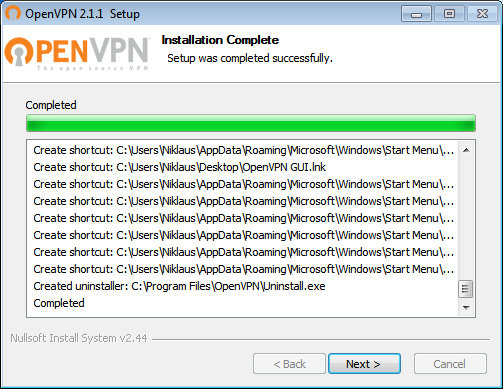
\includegraphics[scale=0.5]{images/OpenVPN_Setup_3}\\


\newpage{}Nach einem weiteren Tastendruck auf {}``Finish'' ist
die Installation beendet.

~

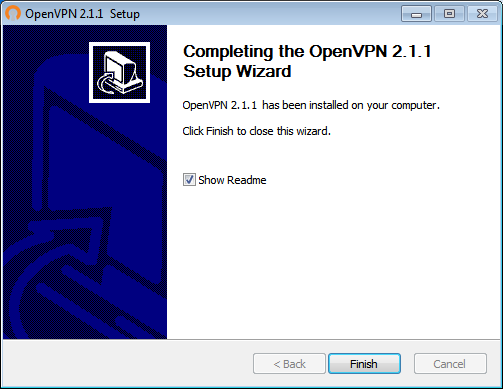
\includegraphics[scale=0.5]{images/OpenVPN_Setup_4}\\



\subsection{Konfiguration (pro Arbeitsplatz)}

Analytica liefert folgende Dateien. Diese m�ssen wie folgt im Ordner
C:\textbackslash{}Program Files\textbackslash{}OpenVPN\textbackslash{}config
abgelegt werden. Dazu brauchen Sie Administratorenrechte und m�ssen
diese Aktion best�tigen.
\begin{enumerate}
\item analytica-ca.crt (�ffentlicher Teil des Schl�ssel von Analytica)
\item Pro Arbeitsplatz (hier die Name f�r die erste)

\begin{enumerate}
\item name\_1.crt (�ffentlicher Teil des Schl�ssel von name\_1)
\item name\_1.key (privater Teil des Schl�ssel von name\_1. Darf nicht weitergegeben
werden!)
\item name\_1.ovpn (Konfiguration von OpenVPN wie IP-Adresse des Analytica-Servers)
\end{enumerate}
\end{enumerate}
Wichtig! Eine Datei wie name\_1.crt darf auf genau einem PC installiert
werden, ansonsten es zu gravierenden Problemen kommt (sprich: Keine
Verbindung mehr m�glich, oder nur wenn nur 1 PC am laufen ist).


\subsection{Erster Verbindungstest}

Zum Testen der Verbindung starten Sie unter {}``Alle Programme..OpenVPN..OpenVPN
GUI''.

Danach sollte Sie in Ihrer Bildschirmleiste ein neues Icon sehen,
das beim Anklicken etwa so aussieht:

~

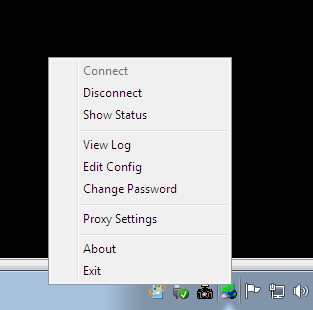
\includegraphics[scale=0.5]{images/OpenVPN_start_1}\\


Dr�cken Sie nun auf {}``Connect''. Falls Ihre Verbindung zu Stand
kommt, erwartet Sie etwa folgendes Bild:

~

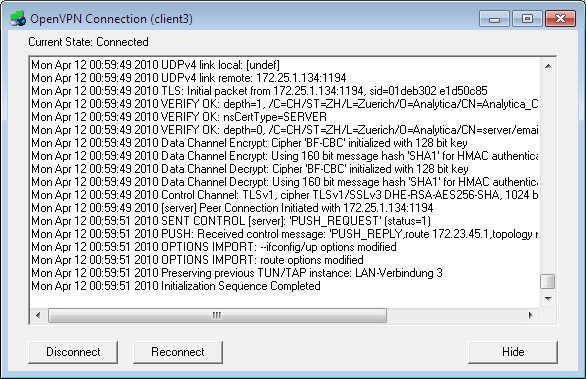
\includegraphics[scale=0.5]{images/OpenVPN_Status_172}\\


Bei Probleme �berpr�fen Sie Ihre Firewall-Einstellungen.


\subsection{Import-Plugin konfigurieren}

Bevor Sie das Plugin benutzen k�nnen, m�ssen in den Einstellung noch
einige Sachen angepasst werden. 
\begin{enumerate}
\item Nach dem Aufstarten von Elexis den Menupunkt Datei..Einstellungen..ausw�hlen.
Datenaustausch..Team-W Import anw�hlen. 
\item Die Felder {}``Adresse des FTP-Servers, FTP User, FTP Password''
gem�ss Angaben von Analytica ausf�llen. 
\item Einen Order f�r die vom FTP-Server herunterzuladnen Dateien erstellen.
Vollst�ndigen Pfadnamen dazu im Feld {}``Download Verzeichnis''
angeben. Auf {}``Apply'' dr�cken. Auf {}``OK'' dr�cken. 
\end{enumerate}

\subsection{Import-Plugin benutzen}

Beim Labor-Blatt benutzen Sie den Menupunkt {}``Import''.

~

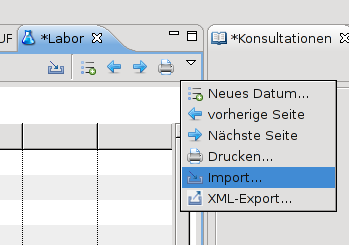
\includegraphics[scale=0.5]{images/Import_4}\\
 Danach k�nnen Sie Daten, entweder aus einer Datei importieren oder
via Plugin alle von Analytica auf dem FTP-Server bereitgestellten
Resultate abholen.

~

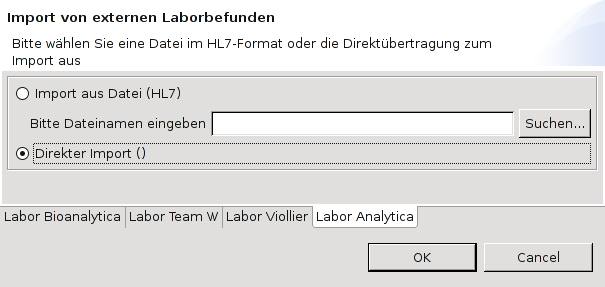
\includegraphics[width=10cm]{images/Import_1}\\


Sie m�ssen die Zuordnung zum Patienten beim Importieren noch best�tigen,
falls diese nicht automatisch festgestellt werden konnte.

Fehlermeldungen:

\begin{lstlisting}
C:\Programme\OpenVPN\config>openvpn.exe --config elexis-1.ovpn
Tue Apr 27 21:12:15 2010 Error: private key password verification failed
\end{lstlisting}


Grund war: {*}.key-Datei war leer, da sie nicht vom Server her gelesen
werden konnte.


\section{Windows-Firewall}

Unter Windows soll man wie folgt die Firewall abschalten k�nnen (via
Registry.key)

\begin{lstlisting}
HKEY_LOCAL_MACHINE\SYSTEM\CurrentControlSet\Services\Tcpip\Parameters IPEnableRouter = dword:00000001
\end{lstlisting}



\section{Wie vorgehen bei Problemen}
\begin{enumerate}
\item OpenVPN-Logdatei �berpr�fen


Die Verbindung ist zu Stande gekommen, falls folgende Zeile gefunden
werden kann


\begin{lstlisting}
Mon Jun 06 16:43:31 2011 Initialization Sequence Completed
\end{lstlisting}


\item FTP-Verbindung �berpr�fen.


Kann mit einem Ftp-Client (z.B. FileZilla von \url{http://www.filezilla.de/})
auf den FTP-Server (z.B. 172.23.45.1) von Analytica zugegriffen werden?\end{enumerate}


\end{document}
